\newpage
\section{Vorgehen}
Es wurde beschlossen, nach SODA \cite{Wikipedia-Scrum} vorzugehen.
SODA ist eine einfache und agile Vorgehensweise zur Entwicklung von Projekten. Dieses Vorgehensmodell wurde von der Hochschule Luzern entwickelt, um den Studenten eine Iterativ/Inkrementelle Vorgehensweise zu bieten, welche trotzdem Zeitlich begrenzt ist. Somit ist es eine Mischung aus dem Wasserfallmodell und Scrum. Scrum wird häufig in der Software Entwicklung eingesetzt, wurde aber ursprünglich aus Studien von Manufakturen wie der Autoindustrie entwickelt \cite{Wikipedia-Scrum-History}.

Da es sich in \acrshort{pren}1 nicht um ein reines Software-, sondern um
ein Interdisziplinäres Projekt handelt, besteht die Gefahr, dass Aufgaben
mit niedrigerer Priorität nicht umgesetzt werden. Aus diesem Grund ist es
wichtig, bereits im Vorhinein mögliche Risiken zu identifizieren und deren Machbarkeit
abzuklären. Dies wurde mittels \nameref{sec:design-thinking} gemacht.

Um zu vermeiden dass niedriger priorisierte Aufgaben nicht vernachlässigt werden,
ist es wichtig ein gutes Backlogmanagement zu erstellen. Das heisst alle Aufgaben/Stories zu definieren (siehe \ref{tab:anforderungsliste}), zu schätzen und zu priorisieren. Damit kann bereits früh festgestellt werden, welche Aufgaben zeitlich umgesetzt werden können.

Es werden wöchentliche Stand-Ups mit dem Coach und allen Teammitgliedern durchgeführt, hierbei wird besprochen, was in der Letzten Woche erreicht wurde, was für Risiken und Hindernisse bestehen (siehe \nameref{sec:risikomanagement}) und was bis zum nächsten Stand-Up erreicht werden soll.

Als Scrum-Board wird Trello\footnote{https://trello.com/} verwendet. Mehr dazu im \nameref{sec:arbeitsjournal}.

\subsection{Organigram}
SODA gibt die folgenden Rollen vor:

\begin{items}
  \item {\bf \acrfull{po}} \\
    Repräsentiert die Kunden des Produktes gegenüber dem Team 
    und ist verantwortlich um einen Business-Value zu generieren.
  \item {\bf \acrfull{sm}} \\
    Entfernt Hindernisse, die das Team an der Producktentwicklung hindern.
  \item {\bf Entwicklungsteam} \\
    Ist für die Entwicklung des Producktes zuständig
\end{items}

\newpage

Die Rollen wurden gemäss dem Organigramm in Abbildung \ref{fig:organigramm} auf das Team verteilt. Natürlich sind im Rahmen der \acrshort{pren}1 Arbeit alle Teammitglieder teil des Entwicklerteams.
Je nach Rolle kann aber mehr oder weniger Arbeit beispielsweise für das Backlogmanagement anfallen.

\begin{figure}[H]
  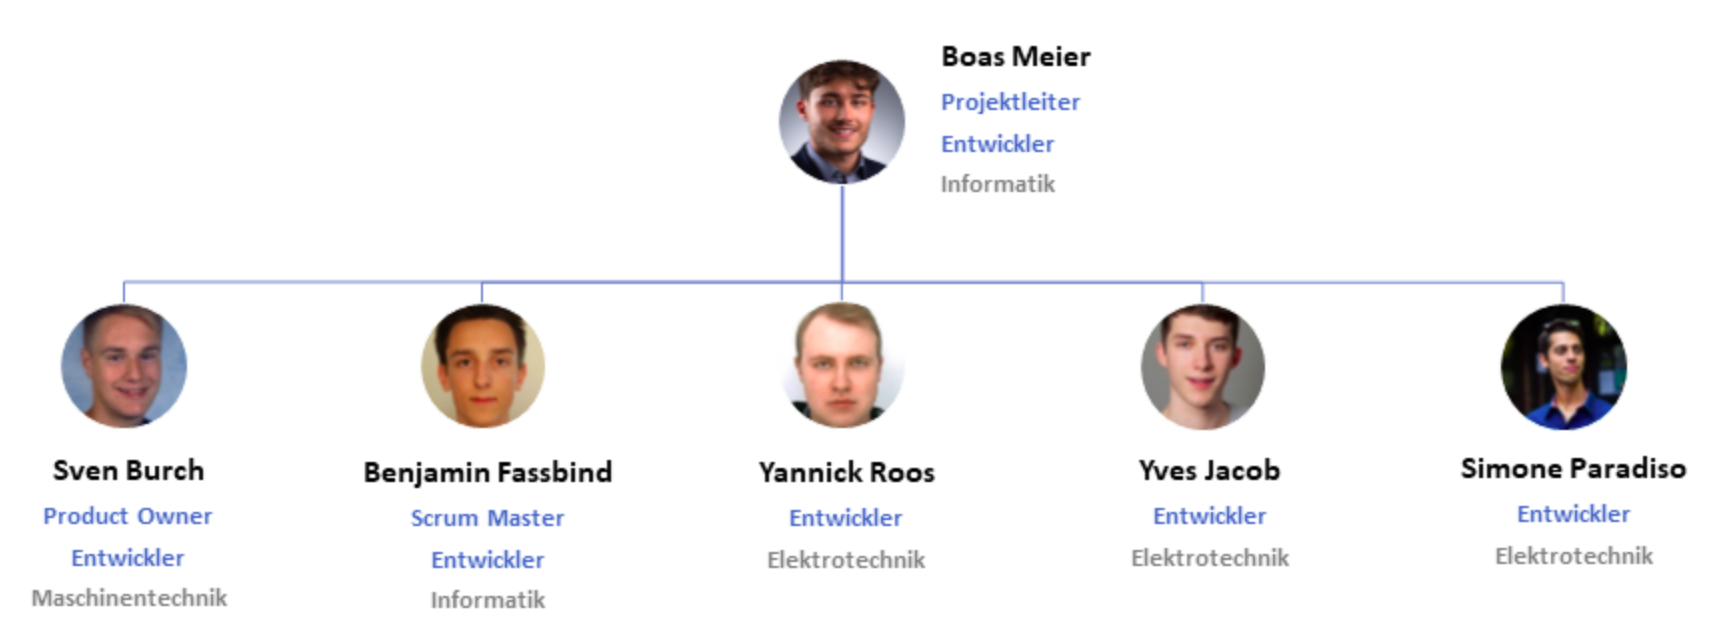
\includegraphics[width=1.0\textwidth]{img/organigram}
  \centering
  \caption{Organigram welches die Projektrollen festlegt}
  \label{fig:organigramm}
\end{figure}

\subsection{Datenaustausch}
Um Daten im Team auszutauschen und gemeinsam Dokumente zu erarbeiten, werden zwei verschiedene Cloud Plattformen verwendet. Jedes Teammitglied hat vollständigen zugriff auf beide Plattformen.

\textbf{OneDrive}\\
Microsoft OneDrive wird verwendet, um Office 365 Dokumente zu verwalten. Dank OneDrive sind diese Dokumente versionskontrolliert und unter allen Mitgliederen synchronisiert. Dies erlaubt eine simultane Bearbeitung.

\textbf{GitHub}\\
Mit Hilfe von GitHub wird der Quellcode versionskontrolliert verwaltet. Es wurden zwei Repositories angelegt. Die Latex-Dokumentation ist unter dem Repository https://github.com/randombenj/hslu-pren1-doc erreichbar und der Quellcode unter https://github.com/randombenj/hslu-pren1.

\newpage

\subsection{Design Thinking}
\label{sec:design-thinking}


Bei Design Thinking \cite{Wikipedia-Design-Thinking} geht es in erster Linie darum, strukturiert 
Ideen für die Umsetzung eines neuen Produktes zu finden. Auch soll das Design Thinking
dabei helfen, zu sehen, ob eine Idee umsetzbar ist. Dies wird dadurch erreicht,
dass sehr einfache (\acrshort{lofi}) Prototypen, beispielsweise aus Karton, 
gefertigt werden, um zu sehen, ob das gewünschte Konzept überhaupt umsetzbar ist.

Ein Ansatz des Design Thinking ist der Double Diamond Prozess. Auch dabei geht es
darum, dass man mit einem Problem konfrontiert wird, im hier dargelegten Fall durch die 
Aufgabenstellung, und versucht dabei die bestmögliche Lösung zu finden.

Die Idee dabei ist relativ einfach: Man unterteilt die Problemlösung in vier Teile.
Als erstes versucht man, möglichst breit gefächert das Problem zu verstehen. Dies geschieht
beispielsweise indem man sich mit den Kunden zusammensetzt und sich mit ihnen über das Problem unterhält.
Danach definiert man eine konkrete Problemstellung auf die man sich fokussiert.
In einer dritten Phase versucht man breit gefächerte Ideen zur Lösung des Problems zu finden.
Diese Ideen können auch durchaus unkonventionell sein, es sollte noch nichts ausgeschlossen werden.
Als nächstes definiert man aus den gefundenen Ideen
die besten, welche sich aufgrund von gewissen Kriterien für die Lösung eignen.
Diese klärt man mithilfe von Prototypen auf die Machbarkeit.
\begin{figure}[H]
  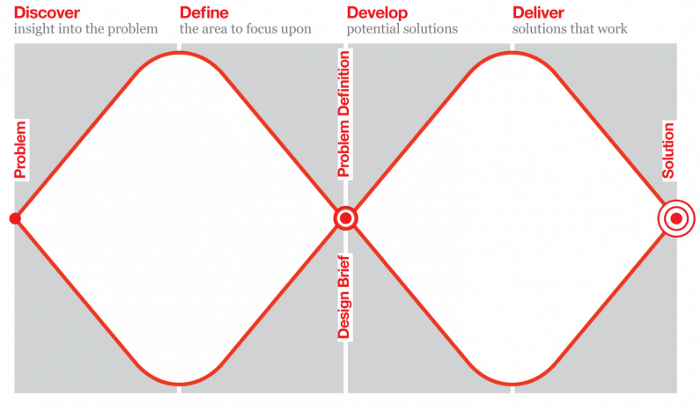
\includegraphics[width=1.0\textwidth]{img/double-diamond}
  \centering
  \caption{Design Thinking mithilfe von Double Diamond}
\end{figure}
  
\subsection{Risikomanagement}
\label{sec:risikomanagement}
Das Risikomanagement wurde iterativ-inkrementell jede Woche in den Stand-Ups durchgeführt. Dazu wurde ein Excel-Template verwendet, welche als Datei dem Anhang beigelegt wird. In diesem Template wurde jedem Risiko einen Risk Score zugeteilt, welcher sich aus Eintrittshäufigkeit multipliziert mit Schadensausmass errechnet. Dieser Risk Score wurde vor und nach der definierten Prävention berechnet. Nachfolgend in der Tabelle \ref{tab:risikomanagement} werden lediglich die wichtigsten technischen Risiken und deren präventiven Massnahmen aufgelistet.

\begin{center}
\begin{table}[H]
    \begin{tabularx}{\textwidth}{l|X|X}
        \textbf{ID} & \textbf{Titel} & \textbf{Vorbeugende Massnahmen} \\ \hline
        R6 & Hindernisse werden nicht erkannt & Möglichst früh Konzept erstellen und mithilfe eines Prototyps testen. \\
        R8 & Roboter erfüllt 4 min Laufzeit nicht & Zeitbudget für einzelne Zustände im Gesamtablauf erstellen und in Evaluation mit einbeziehen. \\ 
        R9 & Komponenten lassen sich nicht kombinieren & Kompatibilität der verschiedenen Komponenten in die Evaluation mit einbeziehen \\
        R10 & Roboter kommt bei seitlicher Traversierung auf der Treppenstufe vom Kurs ab.& Orientierung auf einer Stufe in der Konzeption miteinbeziehen, früh Tests mit Prototypen durchführen.\\
        R11 & Fortbewegungskonzept wird durch die Beschaffenheit der Treppe gestört & Bei Evaluation Untergrund miteinbeziehen. Funktionsmuster bauen bei Unsicherheit. \\
        R12 & Der Roboter gerät bei der Hubbewegung aus dem Gleichgewicht. & Berechnung des Gewichts und des Schwerpunktes.\\
        R14 & Anschlag bei Drehbewegung in der Nähe eines Hindernisses bei minimalem Durchgang von 400 mm. & Lösungskonzept erarbeiten oder Dimension so wählen, dass Rotation immer möglich ist. \\
        R15 & Standfusspostition nach dem Einfahren der Ausleger nicht mehr richtig. & Ansteuerung der Motoren so justieren, dass Ausleger immer richtig eingefahren werden. \\
    \end{tabularx}
    \caption{Risikomanagement}
    \label{tab:risikomanagement}
\end{table}
\end{center}
  
\subsection{Rahmenplan}
Wie in Abbildung \ref{fig:rahmenplan} ersichtlich, hat sich das Team entschieden, das Projekt in vier Sprints aufzuteilen. Somit bilden die drei Testate und die Schlussabgabe die Ergebnisse, welche am Ende eines Sprints vorliegen sollen.

\begin{figure}[H]
  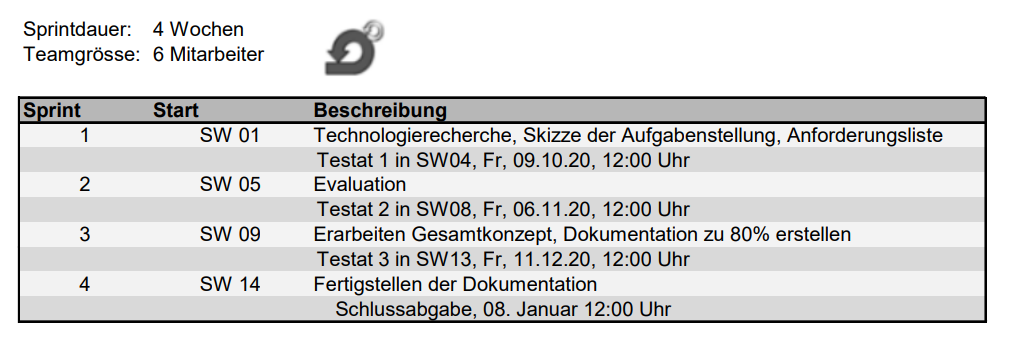
\includegraphics[width=1.0\textwidth]{img/projektmanagement/Rahmenplan.PNG}
  \centering
  \caption{Rahmenplan des Projekts}
  \label{fig:rahmenplan}
\end{figure}

\subsection{Sprintplanung}
Zu Beginn jedes Sprints wurde eine Sprintplanung gemacht. Dazu wurden die Backlog-Items (Epics) mit der höchsten Priorisierung in User-Storys aufgesplittet und in den Sprintbacklog übernommen. 

\subsubsection{Sprint 1}
\textbf{Sprintziel}\\
Das Ziel des Sprint 1 ist, den Roboter in Teilfunktionen zu unterteilen. Weiter soll eine Anforderungsliste und eine Skizze der Aufgabenstellung erstellt werden. Zudem sollen Recherchen bezüglich den einzelnen Teilfunktionen gemacht werden.

\textbf{Risiko-Update}\\
Es sind vier neue Risiken hinzugekommen. Nämlich, dass zu spät mit der Konzeption gestartet wird (R1), dass das Budget überschritten wird (R2), dass nicht fortlaufend dokumentiert wird (R3) und dass sich die Treppendimension ändert (R4).

\textbf{Sprintbacklog}\\
In der Abbildung \ref{fig:sprint-backlog-1} wird der Sprintbacklog gezeigt, welcher in der Sprintplanung erstellt wurde.
\begin{figure}[H]
  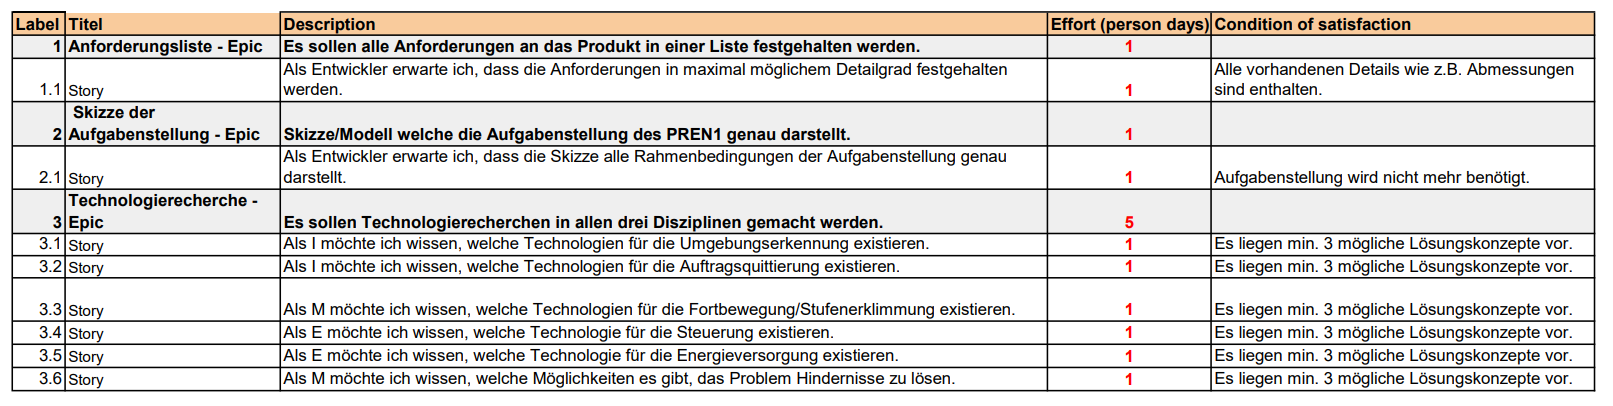
\includegraphics[angle=270,width=0.3\textwidth]{img/projektmanagement/sprint1-backlog.PNG}
  \centering
  \caption{Sprint 1 - Backlog}
  \label{fig:sprint-backlog-1}
\end{figure}

\subsubsection{Sprint 2}
\textbf{Sprintziel}\\
Das Ziel des Sprint 2 ist es, die verschiedenen Lösungsmöglichkeiten welche in Sprint 1 erarbeitet wurden einzugrenzen. Am Ende sollen drei mögliche Grobkonzepte stehen und ein klarer Favorit vorliegen.

\textbf{Risiko-Update}\\
Das Risiko R4, dass sich die Treppendimension ändert ist weggefallen. Da die Treppendimensionen klar spezifiziert und so versichert wurden. Die Risiken, einer Fehlerhaften Evaluation (R5), dass die Hindernisse nicht erkannt werden (R6), dass sich das Team zu früh auf eine Lösung fixiert (R7) und dass der Roboter die maximale Laufzeit von 4 min überschreitet (R8) sind hinzugekommen.

\textbf{Sprintbacklog}\\
In der Abbildung \ref{fig:sprint-backlog-2} wird der Sprintbacklog gezeigt, welcher in der Sprintplanung erstellt wurde.
\begin{figure}[H]
  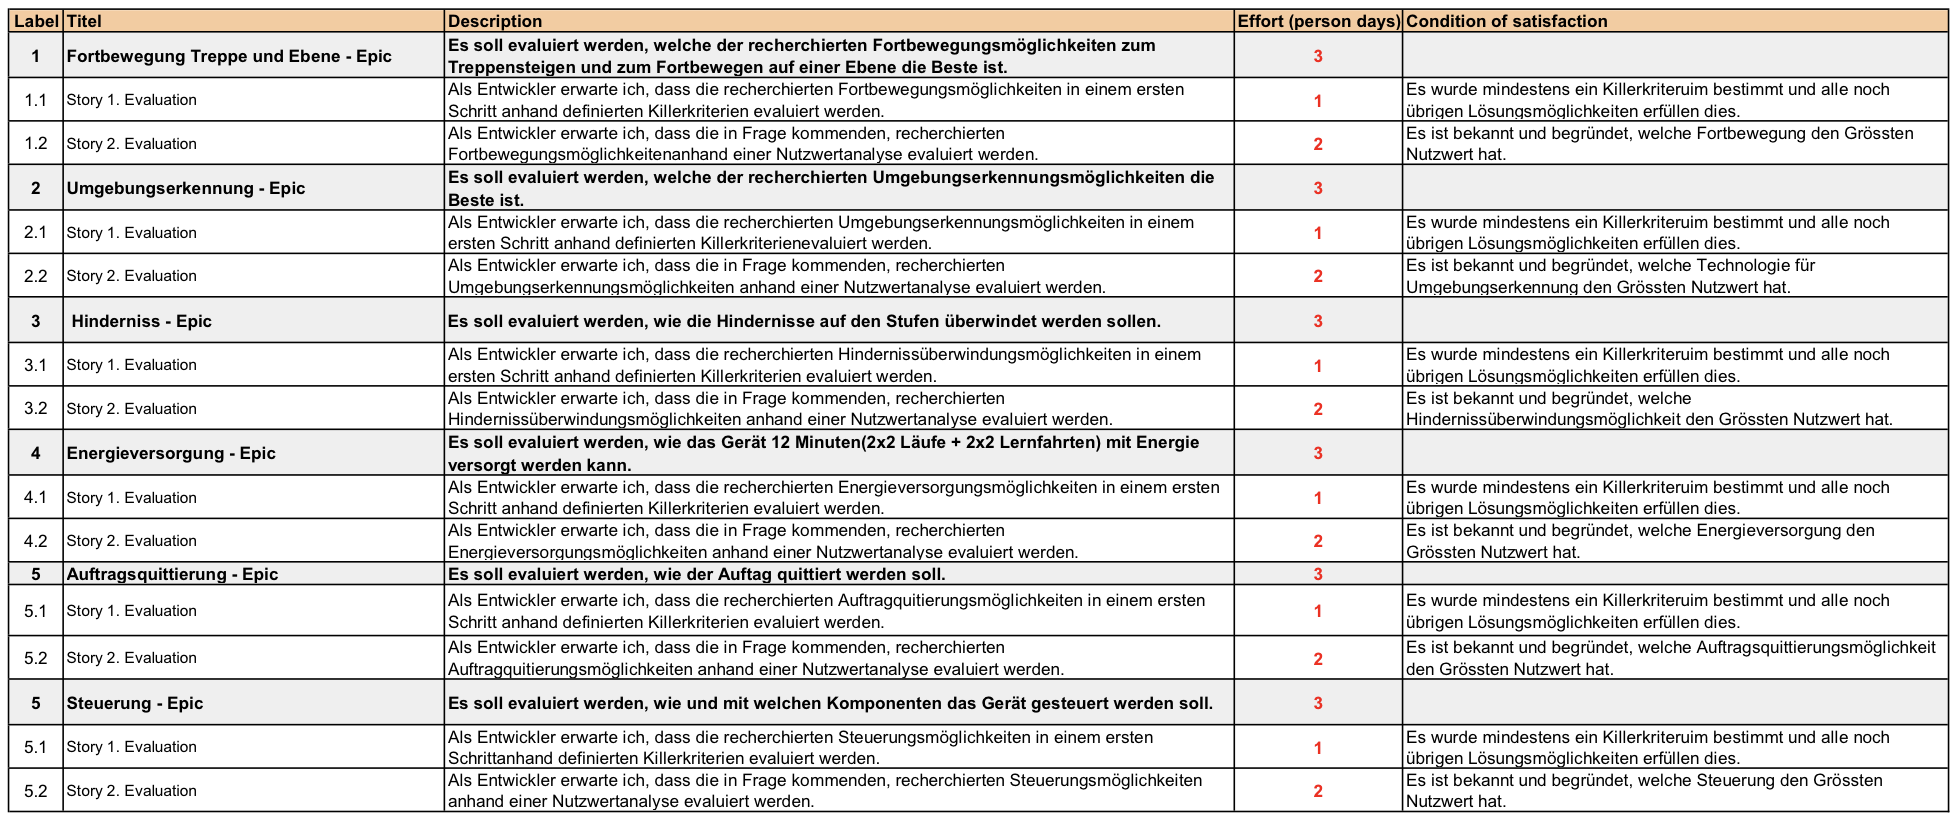
\includegraphics[angle=270,width=0.55\textwidth]{img/projektmanagement/sprint2-backlog2.png}
  \centering
  \caption{Sprint 2 - Backlog}
  \label{fig:sprint-backlog-2}
\end{figure}

\subsubsection{Sprint 3}
\textbf{Sprintziel}\\
Das Ziel des Sprint 3 ist, dass am Ende ein Gesamtkonzept vorliegt. Die Funktionsfähigkeit dieses Konzept ist mit Funktionsmuster untermauert.

\textbf{Risiko-Update}\\
Es sind keine Risiken weggefallen, jedoch neue hinzugekommen. Nämlich, dass sich die Komponenten nicht kombinieren lassen (R9), dass der Roboter beim seitlichen Verschieben eine Treppenstufe runter stürzt (R10), dass das Fortbewegungskonzept nicht mit der Oberflächenbeschaffenheit der Treppe zurecht kommt (R11), dass der Roboter bei der Hubbewegung aus dem Gleichgewicht fällt (R12), dass Teammitglieder aufgrund von Corona ausfallen (R13).

\textbf{Sprintbacklog}\\
In der Abbildung \ref{fig:sprint-backlog-3} wird der Sprintbacklog gezeigt, welcher in der Sprintplanung erstellt wurde.
\begin{figure}[H]
  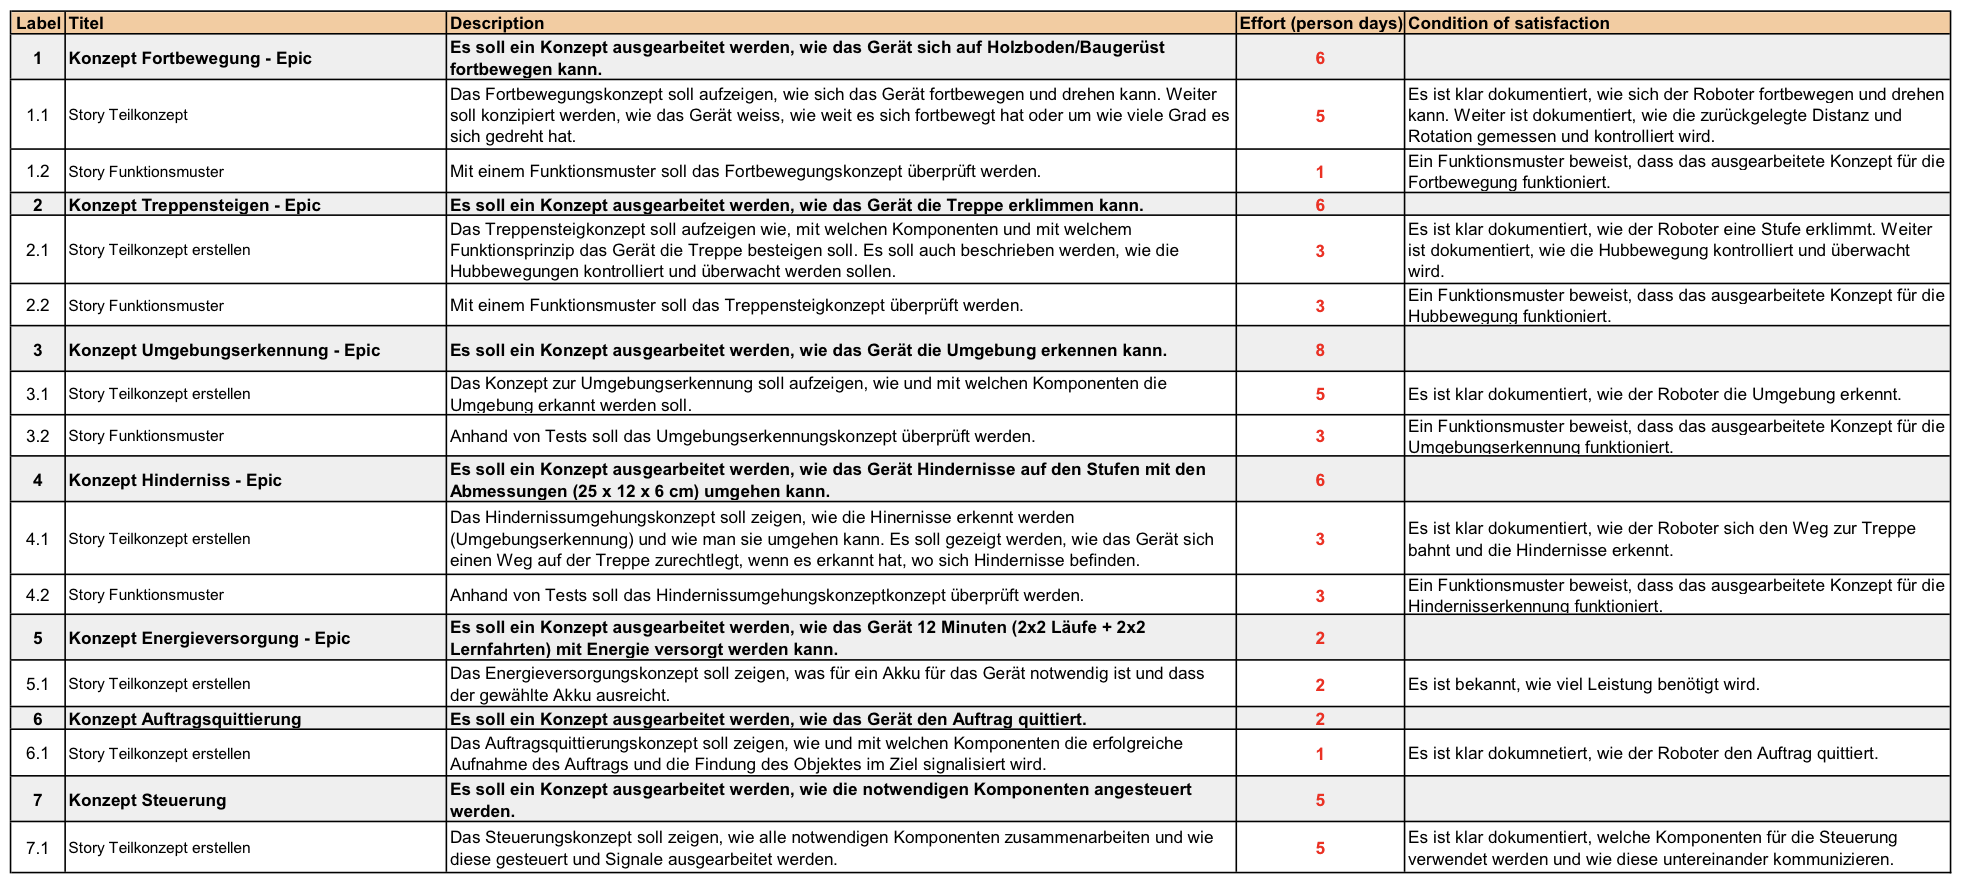
\includegraphics[angle=270,width=0.6\textwidth]{img/projektmanagement/sprint3-backlog2.png}
  \centering
  \caption{Sprint 3 - Backlog}
  \label{fig:sprint-backlog-3}
\end{figure}

\subsubsection{Sprint 4}
\textbf{Sprintziel}\\
Das Ziel des Sprint 4 ist die Fertige Dokumentation gemäss Kriterien.

\textbf{Risiko-Update}\\
Die Risiken R1 und R3 sind weggefallen, da die Dokumentation zu 80\% fertiggestellt und die Evaluation abgeschlossen ist. Neu hinzugekommen ist, dass sich der Roboter beim Drehen auf der Treppe in einem Hinderniss einhakt, wenn der Durchgang die minimal mögliche Breite von 400 mm hat (R14).

\textbf{Sprintbacklog}\\
Für den Sprint 4 wurde kein Sprintbacklog erstellt. Da es im Backlog keine weiteren Items mehr gab.

\section{Arbeitsjournal}
Dieses Kapitel beinhaltet eine Übersicht der Sprints und welche Tätigkeiten 
in diesen gemacht wurden.

\subsection*{Technologierecherche und Anforderungsliste}
\workday
    {1}
    {\ok Meilenstein 1 Erledigt. Alle Tasks abgeschlossen.}
    {
      Es wurde sich intensiv mit der Technologierecherche auseinandergesetzt.
      Dabei wurde versucht, wie im Design Thinking Prozess beschrieben, so breit wie möglich
      zu bleiben.
    }
    {
      Das Testat 1 konnte erfolgreich abgegeben werden mit verschiedenen Technologierecherchen in
      allen Bereichen.
    }
    \begin{figure}[H]
  \centering
  \begin{minipage}[t]{0.45\linewidth}
  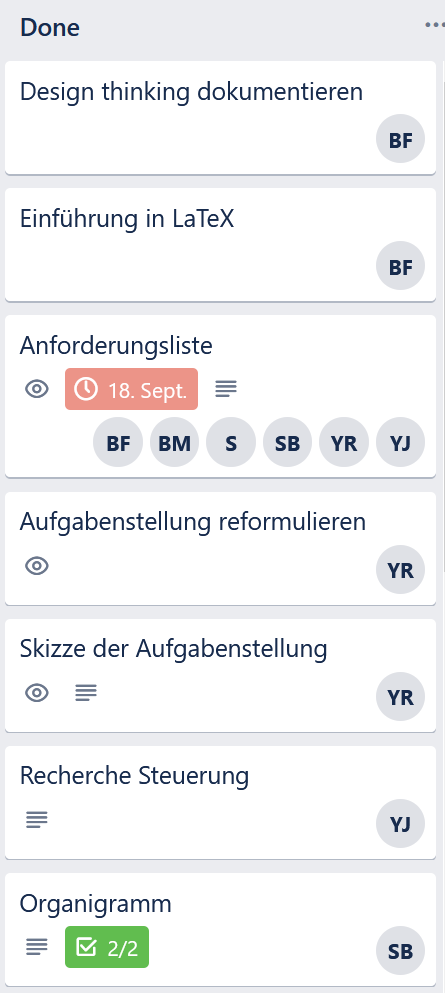
\includegraphics[width=0.7\textwidth]{img/Trello/Trello-Bord_1_Nr1.PNG}
  \caption{Scrum Board des Sprints 1, Teil 1}
  \label{Scrum Board 2.1}
  \end{minipage} 
  \hfill
  \begin{minipage}[t]{0.45\linewidth}
  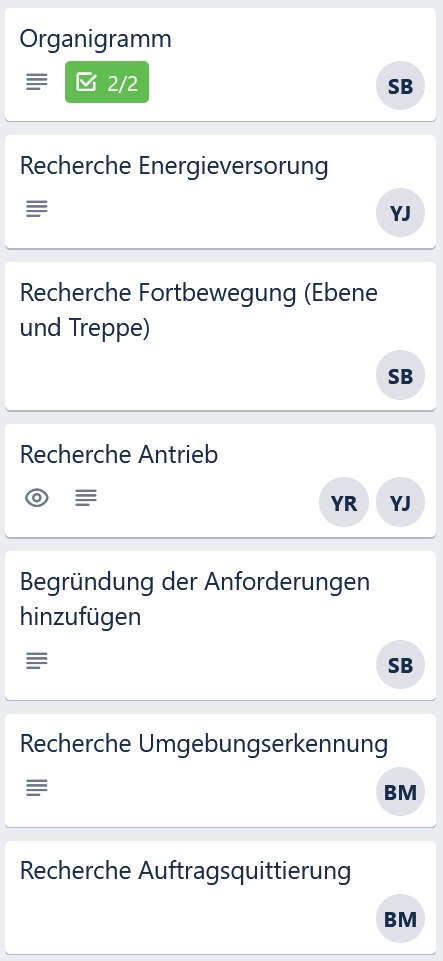
\includegraphics[width=0.7\textwidth]{img/Trello/Trello-Bord_1_Nr2.PNG}
  \caption{Scrum Board des Sprints 1, Teil 2}
  \label{Scrum Board 2.2}
  \end{minipage}
\end{figure}

\subsection*{Evaluation, Auswahl der optimalen Lösungskombination(en)}
\workday
    {2}
    {\ok Meilenstein 2 Erledigt. Bereits mit Meilenstein 3 angefangen.}
    {
      Im Meilenstein 2 wurden aus der Technologierecherche drei Lösungskonzepte erstellt
      und anschliessend evaluiert. Dabei wird der einfachste Ansatz weiterverfolgt. 
      Ganz nach dem Motto ``Keep it simple and stupid''.
    }
    {
      Aufgrund der zügigen Fortschritte bezüglich der ersten Evaluation, konnte rasch zur Evaluation der Teilkonzepte fortgeschritten werden.
    }

    
    \begin{figure}[H]
  \centering
  \begin{minipage}[t]{0.45\linewidth}
  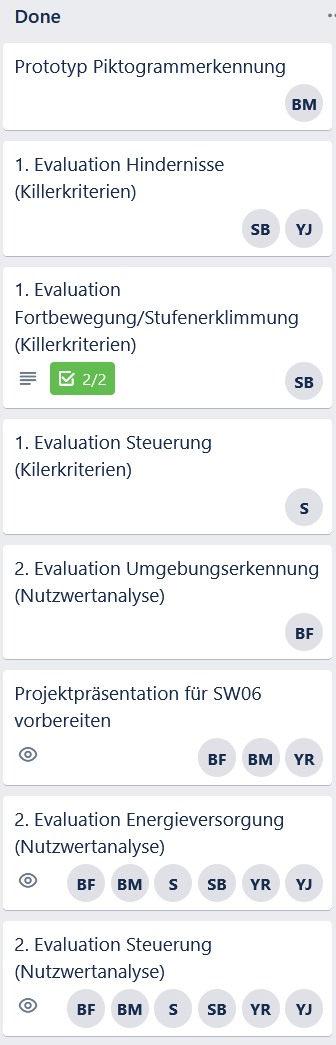
\includegraphics[width=0.7\textwidth]{img/Trello/Trello-Bord_2_Nr1.PNG}
  \caption{Scrum Board des Sprints 2, Teil 1}
  \label{Scrum Board 2.1}
  \end{minipage} 
  \hfill
  \begin{minipage}[t]{0.45\linewidth}
  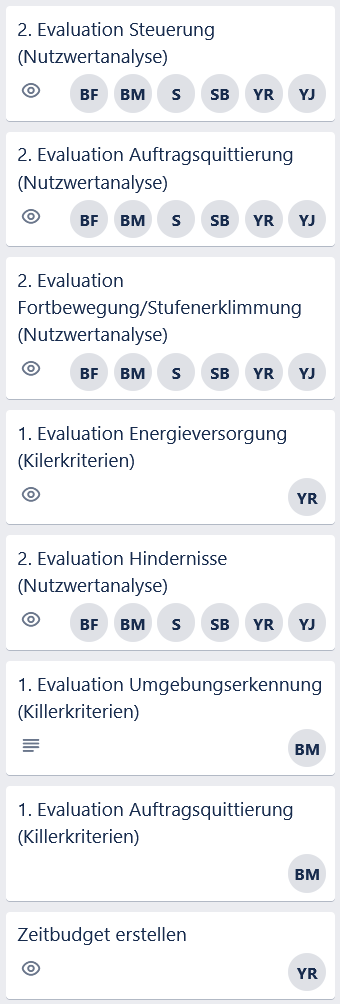
\includegraphics[width=0.7\textwidth]{img/Trello/Trello-Bord_2_Nr2.PNG}
  \caption{Scrum Board des Sprints 2, Teil 2}
  \label{Scrum Board 2.2}
  \end{minipage}
\end{figure}
    
    
    
    
    
    
    
    
    
\subsection*{Freigabe des Gesamtkonzeptes, Dokumentation zu 80\% erstellt}
\workday
    {3}
    {\ok Meilenstein 3 Erledigt.}
    {
      Die Dokumentation wurde soweit zu 80\% fertiggestellt. 
    }
    {
      Die Ideen konnten mithilfe der Funktionsmuster überprüft werden und geben einen verlässlichen Eindruck, wie der Roboter umgesetzt werden kann.
    }

    
    
        \begin{figure}[H]
  \centering
  \begin{minipage}[t]{0.45\linewidth}
  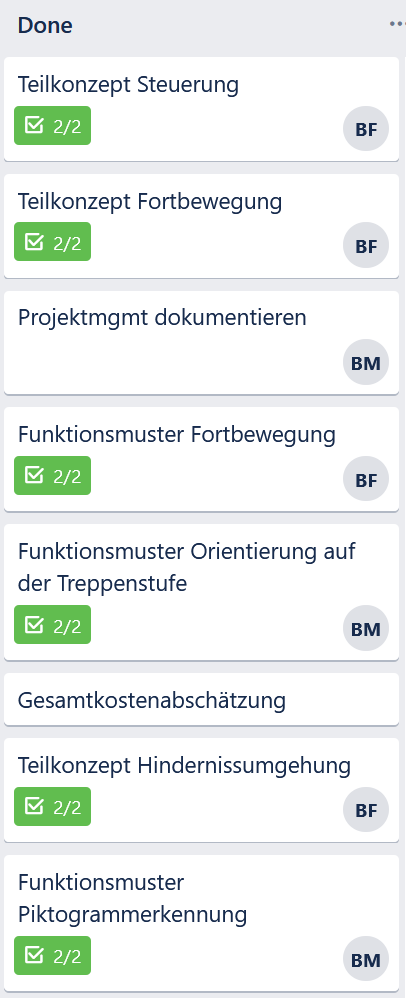
\includegraphics[width=0.7\textwidth]{img/Trello/Trello-Bord_3_Nr1.PNG}
  \caption{Scrum Board des Sprints 3, Teil 1}
  \label{Scrum Board 3.1}
  \end{minipage} 
  \hfill
  \begin{minipage}[t]{0.45\linewidth}
  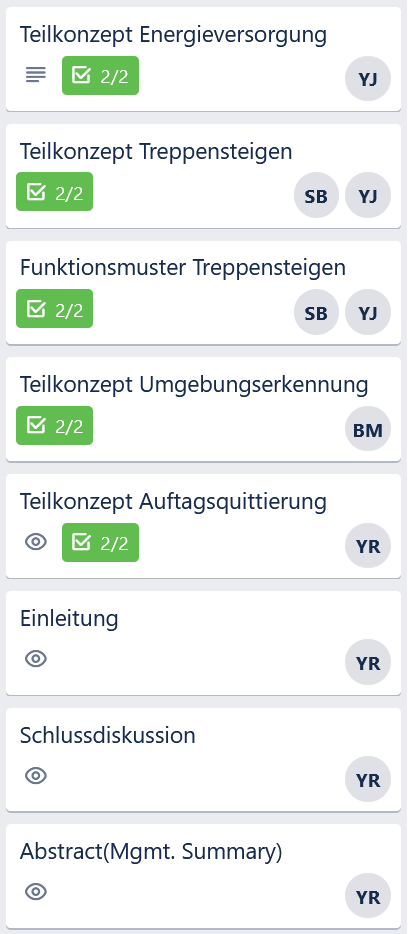
\includegraphics[width=0.7\textwidth]{img/Trello/Trello-Bord_3_Nr2.PNG}
  \caption{Scrum Board des Sprints 3, Teil 2}
  \label{Scrum Board 3.2}
  \end{minipage}
\end{figure}
   